%
% Copyright (c) 1996 Bunyip Information Systems Inc.
% All rights reserved
%
% Archie 3.5
% August 1996
%
%  Configuring the Basic System
%



\Chapter{Configuring the Basic System}
\label{chap:configure}

Now that you have an understanding of the basic structure of the Archie
system, you are ready to continue with the configuration procedure. The
sections in this chapter deal with the necessary installation fine tuning that
will allow you to configure your Archie system to behave appropriately in your
environment.

\section{Configuring the pseudo-domains database}

A pseudo-domain is an alias for a set of domain names. Pseudo-domains are
useful for describing a collection of Domain Name System (DNS) domains which
may not apparently be related (e.g., by spelling). For example, ``.usa'' may be
defined as ``.mil'', ``.com'', ``.edu'' and ``.us''.

The Archie system makes use of pseudo-domain definitions. This is primarily
for convenience in specifying domains as catalog search constraints. The files
\Path{\archie/db/host\_db/domain-db.\symbol{123}dir,pag\symbol{125}}
contain the information where these
definitions are stored. It is the responsibility of individual Archie system
administrators to configure these files as necessary. Note that this database
is visible from remote Archie clients (for example in the anonftp
telnet-client the domains command allows users to see the domain structure of
a server). Users may also search within the catalogs using these pseudo-domain
definitions as restriction criteria.

The tool for modifying this database is the ardomains program, found in
\archie/bin. The input to this program is a file following the format in the
example (see below). The example and the default configuration file are
provided as illustrations of the appropriate format. Some modification will be
necessary to tailor the setup to your Archie server environment.

\begin{center}
\begin{tabular}{lll}
\multicolumn{3}{l}{\#This is a comment line} \\

europe      &  de:ie:pt:es:uk:at:fr:.il:be:nl:ch  & Europe \\

scandinavia  &  no:dk:se    &                       Scandinavia \\

northamerica &  edu:com:gov:us:ca:mil &              North America \\

asia   &      kr:hk:sg:jp:cn:my:tw:in  &          Asia \\

world &       europe:scan:noram:asia    &         The world \\

\end{tabular}
\end{center}

In the example, the pseudo-domain europe has been defined to include the root (top-level) DNS domain names (ISO codes) of the countries of Europe. Pseudo-domain definitions can be nested. So, for example, world is composed of the pseudo-domains europe, scandinavia, northamerica and asia. Short descriptions (265 characters or less) of the pseudo-domains may optionally follow their definition.

When determining if a specific site is a member of a particular pseudo-domain, the Archie system iteratively resolves each pseudo-domain into its base constituents. Thus, world is broken down as follows: 

\path{europe:scan:noram:asia}

and in turn, europe is taken as:

\path{de:ie:pt:es:uk:at:fr:.il:be:nl:ch}

The Archie system then searches to see if any of these are, in turn,
pseudo-domains. This process can be nested to 20 levels.

If an entry cannot be resolved into subcomponents, it is taken ``as is''. Thus
for example, the pseudo-domain uquebec could be arbitrarily defined as

\path{uquebec mcgill.ca:uqam.ca:concordia.ca:umontreal.ca Universities in Quebec}

This provides a list of the various domains within the pseudo-domain of universities in Quebec. The mcgill.ca string cannot be further resolved by the system, so it is considered a base component.

This technique gives both the Archie administrators and users a shorthand notation for specifying domains.

The following points should be kept in mind:

\begin{itemize}
\item
Pseudo-domains must be defined before being used in other pseudo-domains.

\item
On final resolution, the names must match a real DNS domain. The Archie system
makes no attempt to verify the authenticity of the base domains: they are just
used for comparison with site names. A non-DNS name will never successfully
match any data host names stored in an Archie catalog.

\item
The Archie system carries out comparisons of domain strings from right to
left. Thus, m.ca matches both crim.ca and uqam.ca. This can be used to
advantage in constructing domain specification strings. In the example above,
the .il entry differs from the rest by having a preceding period (``.''). This
is so that sites in Israel (``.il'') do not match US military sites (``.mil'').
\end{itemize}


\subsection{Loops in the domain database}

The system will detect domain ``loops''. For example, the entries


\path{canada  qc.ca:on.ca  Provinces in Canada}

\path{on.ca   canada       Ontario}


form a loop: canada resolves into on.ca and qc.ca; on.ca refers back to canada. Archie administrators should try to avoid introducing such loops in their specifications. The ardomains program will identify any it detects.

\subsection{Building the domain database}

To create the domain database, run the program \archie/bin/ardomains on a file containing entries as specified above. The syntax is:

\comm{ardomains [<input file>]}

The \Param{<input file>} should reside in \Path{\archie/etc} for future
reference by Archie programs. By default, the file \archie/etc/ardomains.cf is
used if no file is explicitly given. A sample file is provided in the
distribution for your convenience. Please consult the manual pages for full
details on using this program.



A backup copy of the domains database is maintained in the
\Path{\archie/db/host\_db} directory. Thus, the system is never without a
domain database, even when ardomains is completing the update procedure on the
domain database.



\subsection{Files used by ardomains}

\begin{center}
\begin{tabular}{lll}
File Name & Type & Description \\

\archie/bin/ardomains & Executable & ardomains program \\

\archie/db/host\_db/domain-db.\{dir,pag\} & ndbm data & main domains database
file \\

\archie/db/host\_db/domain-db-new.\{dir,pag\} & ndbm data &
active domains database file (hard link to above) \\

\archie/db/host\_db/domain-db-old.\{dir,pag\} & ndbm data & 
previous version of domains database \\

\end{tabular}
\end{center}


\section{The arserver program}
\label{sec:arserver}

The arserver program provides the external Internet world with a view of the local Archie Host Information Files. It is responsible for responding to queries about the Data Host information as well as performing the protocol negotiations necessary for inter-Archie data exchanges. The server is designed to be run by the UNIX inetd process and thus the file /etc/inetd.conf needs to be modified to inform inetd about the new process.

\alertbox{You must be logged in as superuser to carry out these changes. }



The following single line must be added to the /etc/inetd.conf file with the
correct entry for \Archie \  (the Archie home directory):

\param{arserver stream   tcp  nowait  archuser	 \Archie/bin/arserver  arserver  -l}

The following line should be added to the /etc/services file:

\param{arserver  2710/tcp}

\alertbox{2710 is not a reserved port number. Future releases will probably make use of a reserved port.}



\alertbox{If your system is running the Network Information Service (NIS, formerly called Yellow Pages), additional steps must be taken to incorporate the new services file in your system. Please refer to NIS documentation for details.}



Once these changes have been made, inetd must be notified. The easiest way to
do this is to restart the inetd process. In SunOS 4.X, this can be
accomplished as follows:

\comm{ps aux | grep inetd}

This will extract a line specifying the inetd process, which will look like:


\param{root 162  0.0  0.0  52  0  ?  IW  Oct 23 0:30 inetd}



The process number (\Param{<procnum>}) is the second field (in this case 162). 



Then issue the command:

\comm{kill -HUP <procnum>}

This tells the inetd process to re-read the (modified) configuration file.

For an RS6000 system, however, the following command will perform the necessary updates:

\comm{inetimp; refresh -s inetd}


\section{Invoking arserver}

There are three programs associated with transferring data site information
between remote Archie servers, and internally within your own local Archie
server. They are:

\begin{itemize}
\item arserver

\item arexchange (inter-Archie exchange)

\item arretrieve (local Archie updates)
\end{itemize}


\alertbox{arexchange and arretrieve are currently soft links to the arserver
program; the different names serve to distinguish between tasks to be
accomplished.}



The arserver program is designed to run on demand as connections are made to
it. The arexchange and arretrieve programs, however, are to be run
periodically. This process can be automated through the use of cron (see the
UNIX manual entry cron(8) for details).






\alertbox{All entries for cron should be made in the archuser crontab file, since archuser is the administrative code for the Archie system. Failure to do so may cause problems with improper file permissions for the data files and executable programs.}





All examples in this section will refer back to this sample file. The
arcontrol program will be described in greater detail in ``Controlling the
Update Cycle'' on page~\pageref{sec:control}.



\begin{figure}[!htb]
\begin{center}
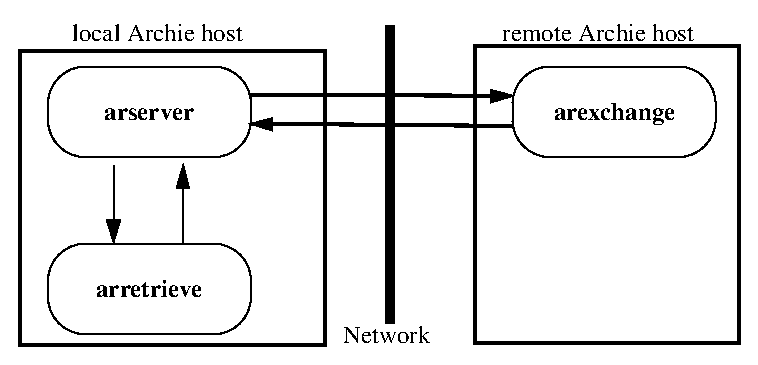
\epsfig{file=figs/exchange.eps,height=2.8in}
\end{center}
\caption{arserver, arretrieve and arexchange relationships}
\end{figure}




%
%
%

\section{Configuration}
\label{sec:configuration}

The arserver, arexchange, and arretrieve commands make use of two
configuration files, with which the Archie system administrator can configure
such things as the data sites that are to be inspected for updating Archie
catalogs (in arretrieve.cf), or the remote Archie servers that are permitted
to participate in an exchange of information (in arupdate.cf).

arupdate.cf is consulted by both arserver and arexchange, while arretrieve.cf
is consulted by arretrieve. Both reside in \archie/etc. Both files have the
same format, but different semantics.






\alertbox{Please note that both configuration files are overwritten by the process accessing them (arretrieve.cf by arretrieve and arupdate.cf by arexchange) at the end of processing. Changes written to the configuration files by the administrator while the processes are running will be lost. }



The Archie site administrator is responsible for configuring these two files
so that the system performs the desired local data retrievals, in addition to
remote exchanges with other Archie hosts.


\section{Configuration decisions}

There are a number of factors to be considered when performing the configuration:

\begin{itemize}

\item What data do you want to store in your local Archie system? This
means deciding which catalogs you would like to serve and from which Data
Hosts you want to pick up the information. For example, you may decide that
you would like to serve all anonymous FTP sites (the anonftp catalog) in
Nigeria, Mongolia and Barbados or provide a webindex catalog for all of
Europe.

\item With whom do you want to exchange inter-Archie data? If you are in a remote location from the data that you would like to serve to your user community, you will probably find that somebody closer is already collecting this data. It is possible that they will be interested in exchanging data with you as well.

\item How often does the data, that you are going to collect yourself or
exchange with a remote Archie site, change? There is no need to exchange
information frequently when the data itself changes infrequently. This also
wastes network bandwidth that could be better utilized.

\item With the current version of the Archie system, the minimum amount of
time between inspections of a Data Host must be greater than the amount of
time required to complete the Update Cycle from the last access. This is
because the Host Information Files are updated as the last step of the Update
Cycle, so the information that would be used to start the next Update Cycle is
not yet available.
\end{itemize}

%
%
%
\section{Choosing Data Hosts}

The worldwide Archie system generally works as a set of independent,
cooperating providers, serving the Internet community. While most Archie
servers are primarily interested in serving their local community on the user
query side of the system, the data host information exchanged between servers
allows each system to provide global data, while only having to monitor a
relatively small number of local data hosts. Each server is free to collect
data directly from any data host desired, however cooperation in the general
data exchange network benefits all concerned and is encouraged.

You may choose to gather data from Data Hosts directly, while obtaining the information about other data hosts from other Archie systems. You should decide which data hosts, if any, you are interested in contacting directly for information and which you would like to obtain from remote Archie servers. Once this decision is made, you can configure your system appropriately.



\alertbox{Bunyip Information Systems coordinates Archie exchanges among its customers as part of the annual support agreement.}



The Archie administrator has significant control over the criteria used to determine what is updated and how often. For example, the Archie system can be configured so that nearby sites are inspected every day while more remote sites are checked every two days. Alternatively, it can be configured so that certain catalogs are updated on even days, and others on odd days. Inter-Archie data exchanges can be configured in a similar fashion.

The next sections will describe the precise format and semantics of the configuration files.


%
%
%
\section{The Retrieval Phase}

As mentioned earlier, the Retrieval Phase is the first step in the Update
Cycle. The local Archie Host Information Files are queried through the use of
the arretrieve command. The query is composed of a set of criteria (or
constraints) that the specified Data Hosts need to meet in order to be
inspected. (For a detailed description of the protocol used between arretrieve
and arserver, see the manual page archie\_protocol). arretrieve then requests
that header records be obtained for any Data Hosts that meet the specified
constraints. These are deposited in the holding directory, where they await
the next phase of the process (refer back to ``Header Records'' in
Appendix~\ref{app:header} for more information about Archie system headers).



The queries that arretrieve sends to arserver are based on the information that the Archie administrator has set up in the arretrieve.cf file. 

\param{<the\_entry>:= <arserver host> <config line>}

\param{<config line>:= <config line> <config> | <config>}

\param{<config>:= <db list> <domain list> <max no> <perms> <freq> <date> <fail>}

where

\begin{TTentry}{<arserver host>}

\item[<arserver host>]
is the Fully Qualified Domain Name (DNS) of the host running the arserver program, to which the arretrieve client will connect. arretrieve and arserver may be run on different machines. However the majority of the time this entry will be localhost.

\item[<db list>]
is the colon (``:'') separated list of Archie catalogs which are to be retrieved.

\item[<domain list>]
is the colon (``:'') separated list of domains and pseudo-domains which the Data Hosts need to match in order to be returned. 

\item[<max no>]
is the maximum number of sites returned matching the criteria.

\item[<perms>]
Permissions (`r'ead or `w'rite). Must be `w' to enable transfer. A value of `r' effectively converts this line into a comment: it will be read but no action will be taken.

\item[<freq>]
A number specifying the minimum number of minutes that are to elapse before contacting arserver with this query again. It may have the modifiers `h' or `d' immediately following the number, specifying that the value is in units of hours or days respectively.

\item[<date>]
Date in YYYYMMDDHHMMSS format. Typically, this specifies the last time that the program performed such a query. In fact, the date is determined by the date of the most-recently inspected site. This is explained more fully in ``Dates in the configuration files'' on page 43.

\item[<fail>]
0. Ignored by arretrieve.
\end{TTentry}

The character \symbol{92} in the configuration file indicates that the entry is continued on the next line of the file.

The following example illustrates the format:

\param{localhost anonftp mcgill.ca:uqam.ca 30 rw 12h 19920703162322 0\symbol{92}}

\param{\hspace{10mm}whois:yp bunyip.com:cndir.org 30 rw 30d 19920603162322 0}

This can be explained as follows:
\begin{center}
\begin{tabular}{|l|p{3in}|} \hline
Field Content & Description \\ \hline \hline

localhost & Contact the arserver program running on the same host as the
arretrieve program. This is the case in almost all Archie installations. \\ \hline
 
anonftp & specifies that information for the anonftp catalog is to be
inspected. Alternatively a `*' may be given, signifying all catalogs. \\ \hline

mcgill.ca:uqam.ca & specifies that they are only to be from sites in the
mcgill.ca and uqam.ca domains. Any pseudo-domain definition may also be
given. Alternatively, a `*' may be given signifying all domains. \\ \hline

30 & specifies that at most 30 sites are to be returned on the retrieval. \\ \hline

rw & The `w' specifies that this line is ``enabled''. The `r' is ignored. \\ \hline

12h & specifies that the program should contact arserver every 12 hours \\ \hline

19920703162322 & specifies the last time arretrieve queried arserver about
this \Param{<database list>/<domain list>} combination. For the initial configuration,
this should be set to your current date and time. The client queries the
server for ``all sites that have not been inspected since \Param{<date>}''. \\ \hline

0 & 
is ignored by the client and should be set to 0 \\ \hline
\end{tabular}
\end{center}

The \symbol{92} signifies that the entry is continued on the next line.

The second (continuation) line gives a configuration for catalogs called whois and yp.

In this way, the Archie system administrator can completely configure how often sites are to be inspected, with full control over what is returned. For example, if one wanted to be responsible for (and query) all Canadian and American sites every day for anonymous FTP information, but European sites only once a week, the configuration could be:


\param{localhost anonftp ca:usa 40 rw 1d 19920810162322 0 \symbol{92} }

\param{\hspace{10mm}anonftp europe 30 rw 7d 19920810162322 0}

This example is only an illustration. In most cases, one would not be responsible for such a large region directly, but would pick up such information through data exchanges with other Archie servers.

The example illustrates a case where the Archie administrator wants to inspect data hosts less frequently than those on the same continent as the Archie server. Specifically, anonymous FTP archive sites within Canada and the United States are to be inspected every day, while those in Europe are to be inspected only every 7 days. 

arretrieve is designed to be run from the cron(8) daemon with a frequency no less than that specified by the shortest interval in the configuration file frequency field.

In the above example, the shortest interval specified is 1 day. The following line would be appropriate in the crontab(5) file.

\param{15 2 * * * \Archie/bin/arretrieve -l -M \Archie/db}

This specifies that cron is to run the arretrieve program at 2:15 every
morning. All appropriate inspections will be started up at this point. In the
example given, North American sites will be inspected each day, and the
European sites will be inspected only once every 7 days. \Archie, is of
course, the Archie home directory. See crontab(5) for full details on the
format of the file.


The arretrieve program does not retrieve any headers.

\NOTE

\begin{itemize}

\item For initial configurations ensure that the date field in the arretrieve.cf file is set to the current date.

\item The first field of the arretrieve.cf file, in almost all cases, will be the special name localhost. Check to make sure that this is the case in your configuration file.

\item Re-check the configuration file to be sure that the syntax is correct and that domains and catalog names can be resolved.

\item Check that arretrieve is a soft link to the arserver binary and that the archuser code has read/execute permissions on the file. 

\item Check that the arretrieve.cf file is has read/write permission for the archuser code.
\end{itemize}



%
%
%

\section{Inter Archie data exchange}

The local arserver program will accept connections from remote arexchange
clients. Similarly, the local arexchange program can contact those remote Archie
arserver programs that give it permission. These permissions are
defined in the configuration file. The default configuration file is
\archie/etc/arupdate.cf. As noted earlier, this configuration file has the
same format as arretrieve.cf, but the semantics are different.

Through the arupdate.cf configuration file, you can set up both symmetric and asymmetric exchange procedures. The symmetric relationship occurs when the connections to your Archie peers are bi-directional: you retrieve data from them and they from you. The asymmetric relationship occurs when either you only retrieve data from them (and not they from you) or vice versa. This is controlled through the use of the \Param{<perms>} field, described below.



\alertbox{Arrangements for the client/server connection must be enabled by the administrators on both sides of the connection for it to be successful. Bunyip regularly posts contact information for Archie servers worldwide on its support mailing lists.}



\subsection{The arupdate.cf file as seen by arserver}

For arserver, the configuration file provides a simple but effective security
mechanism which allows only those sites who have previously been given
permission, by the local administrator, to contact that server.

The fields in the configuration file have the following meanings to arserver:

\begin{TTentry}{<domain list>}
\item[<client host>]
is the Fully Qualified Domain Name (FQDN) of the remote Archie host from which the arexchange client will connect. This may also be an asterisk (``*'') specifying that any remote Archie client may connect.

\item[<db list>]
is the colon (``:'') separated list of Archie databases that the client is allowed to retrieve.

\item[<domain list>]
is the colon (``:'') separated list of domains and pseudo-domains that the Data Hosts need to match in order to be returned. These need to be defined in the local server domains database.

\item[<max no>]
is the maximum number of sites returned matching the criteria.

\item[<perms>]
Either `r' or `rw' specifying the operations the remote arexchange client may
perform. If only `w' is given, the client is not allowed to connect to the server.

\item[<freq>]
Ignored.

\item[<date>]
Ignored.

\item[<fail>]
Ignored.
\end{TTentry}


\subsection{The arupdate.cf file as seen by arexchange}

arexchange, acting from the information in the configuration file, contacts remote Archie servers and queries them about new data which may have been received since contact was last made. If new data exists, the servers negotiate its transfer. It is then placed in the appropriate phase of the Update Cycle and processed identically to the data acquired through the local arretrieve process.

Either the local or the remote Archie system may request that the data being
transferred be in a compressed format. This greatly improves throughput in the
system and is strongly recommended. See the arserver and arexchange manual
pages for full details.

arexchange is designed to be run from the cron(8) daemon by having an entry in the crontab file. The frequency of its invocation should be no less than the shortest interval specified in the configuration file.

The entries in arupdate.cf have the following meanings for arexchange:

\begin{TTentry}{<domain list>}

\item[<server host>]
is the Fully Qualified Domain Name (FQDN) of the remote Archie server. CNAME
records (nicknames) may be used.

\item[<db list>]
is the colon (``:'') separated list of Archie catalogs that the client is to
retrieve.

\item[<domain list>]
is the colon (``:'') separated list of domains and pseudo-domains that the
Data Hosts need to match in order to be returned.

\item[<max no>]
is the maximum number of entries returned matching the criteria. The value 0
is a special case and tells the program to accept as many incoming entries
as the remote server can provide.

\item[<perms>]
Either `w' or `rw' specify the operations that may be performed. If only `r'
is given then the local arexchange client is not allowed to connect to the
specified remote server (\Param{<serverhost>}). That is, \Param{<serverhost>}
may `r'ead local
Archie information, but not `w'rite.

\item[<freq>]
The frequency with which the client is to contact this server about the given
domains and catalogs (given above). It may have the modifiers `h' or `d'
immediately following the number, specifying that the value is in units of
hours or days respectively.

\item[<date>]
Date in YYYYMMDDHHMMSS format. This is explained more fully in below.

\item[<fail>]
The number of failures experienced while trying to contact this server. The
system generates an error condition for the Archie administrator if this
number rises above a pre-determined threshold.

\end{TTentry}


The following is an example of an arupdate.cf file


\begin{tabbing}
\Param{* anonftp ca 0 rw 1 19930321103513 0 } \\
\Param{archie.rutgers.edu anonftp com:mil:edu:net:us:gov 100 rw 1
19930511155204 0} \\
\Param{archie.sogang.ac.kr anonftp asia 0 rw 1d 19930526154304 0 } \\
\Param{archie.univie.ac.at anonftp westeurope:easteurope 0 rw 1d
19930526200058 0 } \\
\Param{archie.uni-linz.ac.at anonftp westeurope:easteurope 0 rw 1d
19930330133007 0 } \\
\Param{archie.switch.ch anonftp westeurope 0 rw 1d 19930524082005 0 } \\
\Param{aries.cc.deakin.oz.au anonftp au 0 rw 1d 19930512124502 0 } \\
\Param{archie2.th-darmstadt.de anonftp de 0 rw 1d 19930524003041 0 } \\
\Param{archie.luth.se anonftp se:dk:no:fi 0 rw 1d 19930527033159 0 } \\
\end{tabbing}



\alertbox{The arserver program will not run until the host databases (in
\archie/db/host\_db) have been created. See the section ``Managing the Host
Information Files'' on page~\pageref{chap:hostmanage} for information on how
to do this.} 



\subsection{Dates in the configuration files}

The initial dates for the configuration files should be set as follows:

\noindent For the arupdate.cf file set the initial date to all zeros. That is,

\param{anonftp se:dk:no:fi 0 rw 1d 19700201010001 0}

\noindent For the arretrieve.cf file, set the initial date to the current date
and time. For example, 

\param{anonftp se:dk:no:fi 0 rw 1d 19940422011500 0}

The times should all be in GMT, but the system will still work correctly if you
just give the time in your local timezone.



\alertbox{As the system is primed you may not get the maximum number of sites
returned until various components in the system synchronize. Running the
programs a couple of times will allow this to happen.} 



When arretrieve and arexchange contact the arserver program, they indicate the
maximum number of sites they want returned, matching the given criteria. For
example, arretrieve might ask for a maximum of 30 sites to be identified for
inspection, when there are in fact 40 that match the criteria. In this case,
the sites are listed in decreasing order of time since last inspection (i.e.,
least-recently inspected, first). The date that is stored in arretrieve.cf
will be the date of the last inspection of the 31st site. This ensures that
the next time arretrieve is run, the sites that were skipped will be
inspected. Typically, this is only an issue when an Archie server is first
brought on-line, and has much catching up to do in terms of inspecting
sites. The is true for the arexchange program, too.

When the number of sites matching the criteria is less than the maximum number
allowed, the date field accurately reflects the date of last inspection. 


\subsection{Updating by ``proxy''}

The arupdate.cf file can be configured to allow ``proxy'' exchanges of information. For example, not every North American Archie server need exchange information with every European server. The global Archie network can be configured so that one site in North America is responsible for picking up information from a particular European site. All other North American sites can be configured to get the information from the delegated proxy server, instead of the European server. This would reduce duplication in inter-continental net traffic. The can be done on a catalog-by-catalog basis.

You may, for example, use the following line in the arupdate.cf file



\param{archie.foo.com anonftp northamerica 0 rw 1d 19930526200058 0}



even if the server, archie.foo.com, is not responsible for the northamerica domain. You can do this if you have arranged with the administrator of this Archie site that, in addition to the data hosts for which that site is directly responsible, you would also like to obtain sites in the northamerica domain.


\section{Controlling the Update Cycle}
\label{sec:control}

The arcontrol process (described in ``The Update Cycle in detail'' on page~\pageref{sec:update}) is responsible for coordinating the entire Update Cycle. It too is invoked in different modes depending on the required functionality. 

\begin{itemize}
\item  With the -r command line switch, it runs in retrieval mode, coordinating the Data Acquisition Component of the Update Cycle.

\item  With the -p command line switch, it runs in parse mode, performing the necessary functions to parse the waiting data files.

\item Finally, with the -u command line switch, it runs in update mode. The data is finally entered into the appropriate Archie user catalogs and the system's Host Information Files are also modified to reflect the new information.
\end{itemize}


In all cases, arcontrol's main task is to scan the holding directory for data files of appropriate type for the particular Cycle phase, perform any necessary pre-processing (uncompressing data files for example) and invoking the correct program for that phase and that catalog. arcontrol is designed to be run from the crontab file of archuser. The relevant entries from the example crontab file are:



\param{0 3,15 * * * <archie home>/bin/arcontrol -r -l }

\param{30 3,15 * * * <archie home>/bin/arcontrol -p -l}

\param{45 3,15 * * * <archie home>/bin/arcontrol -u -l}



These entries specify that, at 3:00 and 15:00, arcontrol is to run in Retrieve Mode. Thirty minutes later it runs in Parse Mode, to process some, if not all of the data files retrieved in the previous phase. Finally at 3:45 and 15:45 it is run in Update Mode, the final step of the Update Cycle.

In Retrieval mode the processing is performed asynchronously and any number of copies of the arcontrol program can be running.


%
%
%

\section{Temporary and Lock files}

The current version of arcontrol performs all pre-processing on data files
first, before invoking the appropriate sub-processes. These files have the
``temporary'' suffix designator ``\_t''. In order to prevent concurrent update of
any particular catalog, a series of lock files are created. These files reside
in the \archie/db/locks directory and are called:

\param{<catalog\_name>\_lock}

These files remain for the duration of the update process and contain the name
of the process creating them, the time created and the name of the datafile
being processed. They will be removed with the successful completion of the
update. The lock file will not be removed if either of the following
situations occur:

\begin{itemize}
\item
The update process which created the lock file is killed or aborts prematurely. An abort can occur if subprocesses performing the update themselves are terminated or aborted.

\item
The host system is rebooted or crashes, thereby prematurely terminating the update process.
\end{itemize}


%
%
%

\section{Host shutdowns and crashes}

Abnormal termination of the update procedure can occur if the host system crashes or is rebooted during the update. If this happens one should do the following:

\begin{itemize}
\item Check the integrity of the catalog in question. Depending on the type of catalog, various programs may be available to do this. See the chapters in this manual, describing the individual catalogs, to determine the exact procedure appropriate to that catalog.

\item If the catalog is corrupted and can be fixed, apply the appropriate
procedures for that catalog to effect the repair.

\item If it is not corrupted (or has been fixed), remove the lock file.

\item If you would like to reprocess data files that did not get processed because of the abnormal termination, then the update\_t files should be renamed without the ``\_t'' suffix. They will then be processed during the normal Update Cycle.
\end{itemize}


\alertbox{It is the responsibility of the Archie system administrator to recover from a crash.}

%
%
%

\section{More disk/less time}

System administrators should take note of the ``-U'' command line option for
the arcontrol program.

In order to conserve disk space, arcontrol normally compresses the data in the
files processed during the Update Cycle.  If you have enough disk space, you
may achieve a significant speed-up by specifying this option, which disables
the compression and decompression of the data during processing.  See the
arcontrol manual page for further details.

%
%
%

\section{Monitoring the System}
To assist in the process of Archie system administration, the system can be
configured to mail regular reports describing its activities. This is
accomplished by creating a file called mail.results in the \archie/etc
directory. This indicates to the system that it is to keep track of its
activities in special files also located in the \archie/etc directory. These
are mail.fail, mail.success, mail.add, mail.retr, mail.parse and
mail.delete. In order to have the results mailed back to you, edit the file
\archie/bin/mail\_stats and, if necessary, change the line:

\param{MAIL\_PGM=/usr/ucb/mail}

to reflect the full pathname of the mail program you would like to use. 

Whichever executable is used to define \Param{MAIL\_PGM}, it must accept a ``-s''
command line switch with the subject of the mail as its parameter.

Also, the line: 

\param{ARCHIE\_USER=archuser}

should describe the valid address to which the results should be mailed. Finally, an entry in the archuser crontab file must be made, in order to run the mail\_stats program (a frequency of once a day should suffice).



If you are not receiving any mail from the system. \NOTE 


\begin{itemize}
\item
Check the archuser crontab file to ensure that the mail\_stats program is being run.

\item
Check that your \Param{MAIL\_PGM} variable is correctly defined and is a fully specified pathname.

\item
Check that the address to which the program is sending mail is correct, by
manually mailing a test message to that address and verifying tha it arrives.

\item
Make sure that the update cycle is in fact running, by checking the crontab
entries and log entries, as well as performing manual invocations of the
arcontrol program.

\end{itemize}


The tool ``daily-admin'' is provided for managing the various log files. The
purpose of this tool is to control the amount of disk space used by the logs,
as well as reporting statistics to the maintainer of the server and to
Bunyip. The package ``daily-admin'' compresses the log file and copies it to
the logs subdirectory ``history'', keeping a certain number of history logs on
the system.

Note that the script will now process all files that have the extension
\Param{.log} present in the directory \Path{\archie/logs}. Also an extension
having the format \Param{YYMMDD} is used to archive the files. \new
 
The ``gzip'' program is used to compress the log files. If it is not found
the ``compress'' program is used instead. It handles the logs in \archie/logs
and \archie/pfs/pfs.log differently. In the case of archie.log and email.log,
the package compresses the log file and keeps the last 32 copies on the
system. In the case of pfs.log, the logs are separated by day, and each day's
information is compressed. This information is kept for 6 months. Since
the programs consist of shell scripts and Perl scripts, these values may be
changed.



We hope that you will use this tool to help you manage your site and at the
same time help us to maintain statistics on Archie usage, as well as follow
the progression of your site. You should add the following line in the
archuser user's crontab.



\param{\# For logs and stats}

\param{5 0 * * * <archie-home>/scripts/daily.admin}



The script should run at around midnight local time. You may use a ``-c'' flag
to send also a copy of the stats to an additional email address, as shown
below.



\param{\# For logs and stats}

\param{5 0 * * * <archie-home>/scripts/daily.admin -c you@your.domain.name}


\subsection{Statistical Package}

We have written a few programs that are called by daily.admin
to process the log files and extract a certain amount of information.
This information can then be presented to the users via HTML pages.
You may take a look at the stats package at
\Path{http://archie.bunyip.com/archstats.html} before installing it on your
system.

        Basically this package can be used in two ways, either while
using HTML tables, making the transfered documents quite big, or by using
pregenerated gif files. In order to generate the gif files, you will need
to have Perl 5 installed on your system and the GD extension module library.


Steps to setting up the package:


  - Go through the file archie-include.pl and do the necessary
    configurations.  These configurations are necessary to both the
    management tools and the CGI scripts that display the statistics.

  - Verify that the file archie-include.pl accompanies the rest of the
    perl scripts (in the same path). It also has to coexist with
    archie-stats-cgi.pl which will be placed in the CGI directory of
    your Web tree.

  - For the daily management routines introduce some lines to Archie's
    crontab as follows:

\param{5  0 * * * /archie/scripts/daily.admin}

\param{5  1 * * 1 /archie/scripts/archie-periodical-stats.pl -w -D -p
/archie/stats -P /archie/stats}

\param{5  1 1 * * /archie/scripts/archie-periodical-stats.pl -m -D -p /archie/stats -P /archie/stats}


  - For the statistical viewing scripts, place archie-stats-cgi.pl
    (along with archie-include.pl as a symbolic link) in the cgi-bin
    directory of the http server you are running on the Archie machine.
    Read note [1].

  - Create a directory for the GIF files on your web server's
    tree. This directory is linked to the directory in the archie tree
    that holds the GIF images created daily.  For example, if the stats
    images that are created reside on ~archie/stats, then you create a
    directory in your http server's images path. This directory is in
    turn linked to ~archie/stats.

  - For the HTML file "archstats.html", make the necessary changes to
    the URL links in the files.  Pay special attention to the "action"
    field such that it reflects the CGI script's (archie-stats-cgi.pl)
    location.

  - For the main Archie search page that usually accompanies the main
    distribution (cgi/html/archie.html), we have added a link to the
    statistics page right at the bottom of the page.  This link is
    relative and is commented out. You will have to uncomment it and to
    decide how to represent it depending on your Web tree setup.


  [1] Note on the script that is used to display the stats on web browsers:


   There is one script that performs the direct CGI interface to the
   statistical database and it is "archie-stats-cgi.pl". This script should
   exist on the http server's tree. However, this script calls
   "archie-display-stats.pl" to display the statistical graphs. This later
   script resides where the rest of the archie scripts reside (normally in
   ~archie/scripts).

   If you have perl5, and can install the GD package for perl5
   (\Path{http://www.boutell.com/gd/}) then you may want to set the variable
   \Param{allow\_gifs} in \Param{archie-include.pl} to 1.  This will let you create the
   GIF files daily/weekly/monthly and will allow you to view them
   automatically.

   If you don't have perl5 or cannot install the perl library GD.pm then you
   will have to set the value of \Param{allow\_gifs} in
   \Param{archie-include.pl} to 0. This will result in the display of the
   statistical histograms in table formats instead of GIF files.



\section{Administrative addresses}


Archie site administrators need to set up an administrative account for bug
reports, comments, suggestions, additions and deletions to the catalogs,
etc. Make an entry for archie-admin in the \Path{/etc/aliases} file, pointing
to the person or persons responsible for the administration of the server. For
example:

\param{archie-admin: myaddress@your.domain.name}

%
%
%

\section{Moving right along}

We've talked about what you'll need to do to configure the retrieval and
exchange components, now we'll take a look at the setup to enable users to use
the catalogs.

